\newpage
\section{Calculations for Graphene}

Placed over the nanostructure described in figure \ref{fig:lumerical} there is a layer of graphene under tensile strain. This layer is sucked into the cavity for about \SI{5}{nm} according to \cite{heeg}. To get a realistic estimation about the location of the graphene layer a 3D modelling software with cloth simulation will be used.

\subsection{Simulating the layer of graphene}

\begin{figure}[!h]
  \centering
  \begin{subfigure}{0.6\textwidth}
    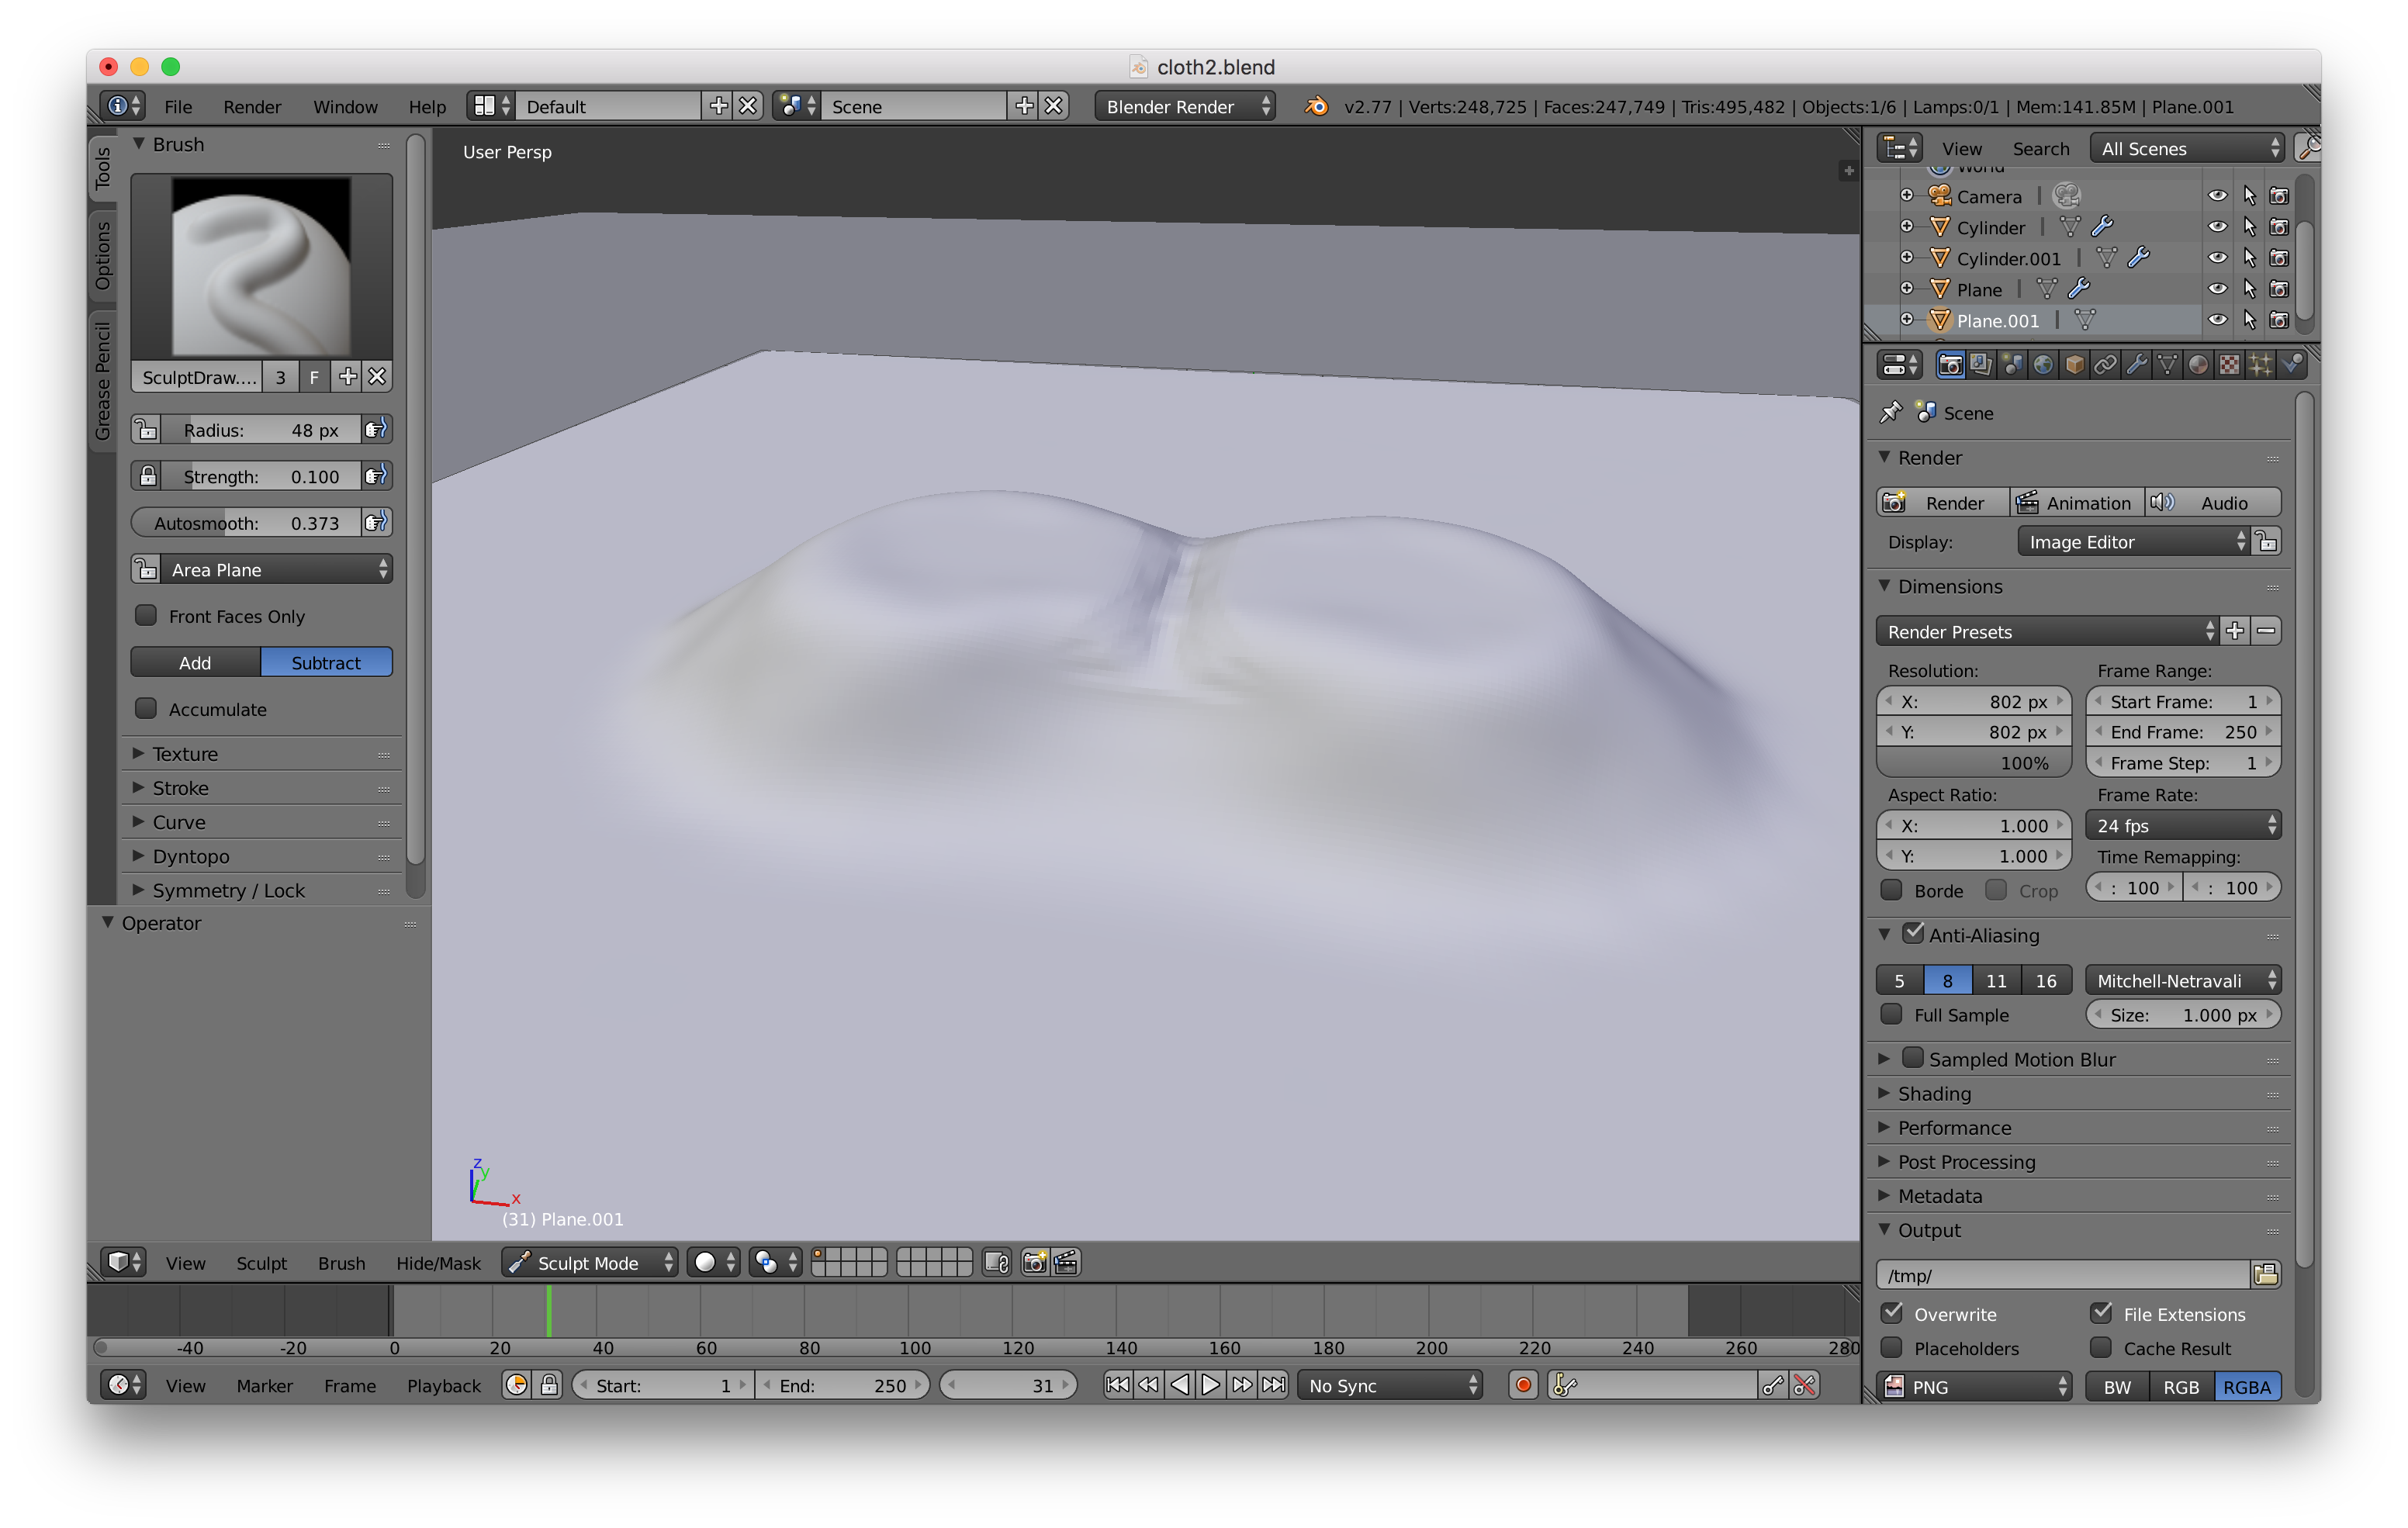
\includegraphics[width=\textwidth]{./images/blender.png}
    \label{fig:blender}
  \end{subfigure}
  ~
  \begin{subfigure}{0.35\textwidth}
    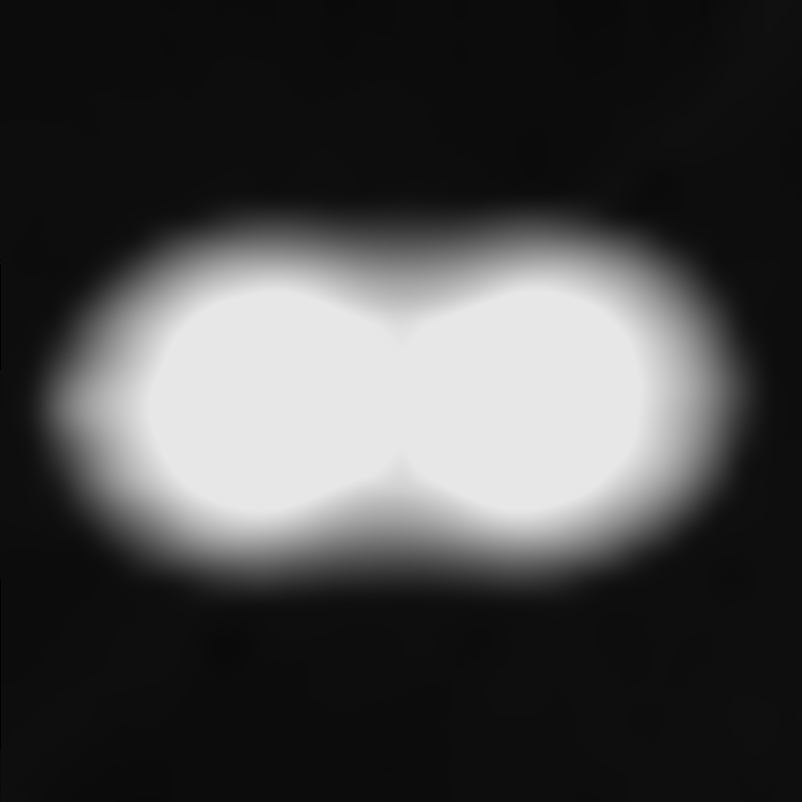
\includegraphics[width=\textwidth]{./images/map.png}
    \label{fig:heightmap}
  \end{subfigure}
  \caption{\textbf{(a)} Cloth simulation in Blender 2.7. An elastic material is dropped on 2 cylinders with a radius of \SI{50}{nm}. \textbf{(b)} A generated heightmap after rendering. Black corresponds to 0, white to maximum height.}
\end{figure}

Using the 3D modelling software Blender 2.7 a simulation of cloth falling on 2 cylinders is used as a basis for the location of the graphene layer. As visible in figure \ref{fig:blender} two cylinders of \SI{45}{nm} height and \SI{50}{nm} radius (gold nanostructures plus chrome interlayer) are placed on an infinite plane. Next up a 1nm thick plane is placed on top and cloth simulation is enabled for this layer.

After the simulation has finished with the cloth like material the results are compared to figure 1c of \cite{heeg}. This is repeated with tweeked properties of the material until the simulated 3D model matches estimated position of the graphene layer. Because no material caused the layer to be sucked into the cavity the manual sculpturing tool is used to move the layer down into the cavity. The resulting 3D model is shown in figure \ref{fig:blender}.

To import the simulated structure into Matlab for further calculations an intermediate step is used. A camera in the scene is setup to point down at the structure with a special light source that illuminates the simulated layer according to it's $z$ value. The highest value is represented as white while black represents the base plane. All other values are projected linearly in the gray colorspace, effectively creating the heightmap shown in \ref{fig:heightmap}.

This heightmap can now be imported as a two dimensional matrix of height values:
\begin{minted}{matlab}
  classdef map
     properties
         values
     end
     methods
         function obj = map(name, scale)
            image = double(imread(name));
            if ndims(image) == 3
              image = 0.2989 * image(:,:,1) + 0.5870 * image(:,:,2) +
                0.1140 * image(:,:,3);
            end
            max_value = max(reshape(image, 1, []));
            obj.values = image ./ max_value .* scale;
         end

         function height = height(obj, x, y)
            height = obj.values(x, y);
         end
     end
  end
\end{minted}

This imports an image, converts it to grayscale if needed, normalizes the values to be between 0 and 1 and then scales the heightmap with a factor. For this to work the image has to have the same resolution as the simulation (401 datapoints in the $x$ and $y$-axis for this case).

This calculation is using a scale factor of $47$ so the graphene layer is hovering \SI{2}{nm} above the gold structure. This is done to mitigate the lightning effects at the discretised surface of the nano structure.
